\documentclass[11pt,letterpaper]{article}
% isms-27000-style.tex
% Suite preamble for the ISO/IEC 27000/27001/27002 ISMS engineering suite.
%
% RECONSTRUCTION PROVENANCE: the ten uploaded suite documents load a shared
% preamble with `\input{style.tex}`, but no `style.tex` was present in the
% upload batches or anywhere in this repository's history. This file is a
% documented, suite-specific reconstruction inferred from the macros, colors
% and environments the documents actually use (colors navy/teal/graytext/pale;
% tag commands \SourceTag, \EngineeringTag, \SourceNote{..}; breakable
% tcolorbox callouts; color-striped longtables; TikZ flow diagrams). It is
% NOT the recovered original style; the original visual design is unknown.
%
% pdfLaTeX only.
\usepackage[T1]{fontenc}
\usepackage[utf8]{inputenc}
\usepackage{lmodern}
\usepackage{microtype}
\usepackage[letterpaper,margin=0.9in,headheight=15pt]{geometry}
\usepackage[table]{xcolor}
\definecolor{navy}{HTML}{14355A}
\definecolor{teal}{HTML}{0A7580}
\definecolor{graytext}{HTML}{55616E}
\definecolor{pale}{HTML}{EFF5F7}
\usepackage{amsmath,amssymb}
\usepackage{array,booktabs,longtable,tabularx,multirow}
\usepackage{enumitem}
\usepackage[most]{tcolorbox}
\usepackage{tikz}
\usetikzlibrary{arrows.meta,positioning,shapes.geometric,fit,calc}
\usepackage{needspace}
\usepackage{titlesec}
\usepackage{fancyhdr}
\usepackage{lastpage}
\usepackage{hyperref}
\hypersetup{colorlinks=true,linkcolor=navy,urlcolor=teal,citecolor=navy,pdfauthor={ISMS Engineering Documentation Suite},pdfsubject={Original supporting guidance for ISO/IEC 27000, 27001 and 27002}}
\setlength{\parindent}{0pt}
\setlength{\parskip}{5pt plus 1pt}
\setlength{\emergencystretch}{2em}
\renewcommand{\arraystretch}{1.18}
\setlist[itemize]{itemsep=2pt,topsep=3pt,leftmargin=1.5em}
\setlist[enumerate]{itemsep=2pt,topsep=3pt,leftmargin=1.7em}
\titleformat{\section}{\Large\bfseries\color{navy}}{\thesection}{0.7em}{}[\vspace{-3pt}\color{teal}\titlerule]
\titleformat{\subsection}{\large\bfseries\color{navy}}{\thesubsection}{0.6em}{}
\titleformat{\subsubsection}{\normalsize\bfseries\color{teal}}{\thesubsubsection}{0.55em}{}
\pagestyle{fancy}
\fancyhf{}
\fancyhead[L]{\sffamily\footnotesize ISO/IEC 27000 series | ISMS Engineering}
\fancyhead[R]{\sffamily\footnotesize\color{graytext} Independent companion}
\fancyfoot[L]{\sffamily\scriptsize Original explanatory material; consult the licensed standards}
\fancyfoot[R]{\sffamily\scriptsize\thepage\ / \pageref{LastPage}}
\renewcommand{\headrulewidth}{0.3pt}
% Inline provenance tags used throughout the suite: \SourceTag marks
% statements grounded in the standards; \EngineeringTag marks original
% engineering interpretation. Both are zero-argument label commands.
\newcommand{\SourceTag}{\textsf{\footnotesize\bfseries\color{navy}[Standard]}~}
\newcommand{\EngineeringTag}{\textsf{\footnotesize\bfseries\color{teal}[Engineering]}~}
\newcommand{\SourceNote}[1]{\par\smallskip{\footnotesize\color{graytext}\textit{Trace: #1.}}\par}

\begin{document}
\pagenumbering{roman}
\begin{titlepage}
\vspace*{1.2in}
{\color{teal}\rule{\textwidth}{4pt}}\par\vspace{20pt}
{\Huge\bfseries\color{navy} Cloud Security and DevSecOps Automation}\par\vspace{18pt}
{\Large\color{graytext} Shared responsibility, control gates, evidence pipelines and measured assurance}\par\vspace{1.3in}
{\large ISO/IEC 27000:2018 $\vert$ ISO/IEC 27001:2022 $\vert$ ISO/IEC 27002:2022}\par
\vfill
\textbf{Independent educational and engineering implementation reference}\par
Version 1.0 $\cdot$ October 2026\par
{\small Original explanatory material. Source standards are copyrighted; consult licensed originals for authoritative requirements.}\par
\end{titlepage}
\tableofcontents\clearpage\pagenumbering{arabic}
\section{Cloud and delivery shared responsibility}
ISO/IEC 27002:2022 5.19--5.23 addresses supplier and cloud service security, while Clauses 8.8, 8.9, 8.15--8.16 and 8.25--8.33 inform platform and software operations. Shared responsibility must be specific to the actual service, contract and assessed risk; do not assume responsibility transfers to a provider merely because a service is managed.
\section{Reference cloud platform control plane}
\small\rowcolors{2}{pale}{white}\begin{longtable}{p{.24\linewidth}p{.42\linewidth}p{.28\linewidth}}
\rowcolor{navy} \textcolor{white}{\textbf{Control plane}} & \textcolor{white}{\textbf{Engineering capability}} & \textcolor{white}{\textbf{Suggested evidence}}\\
\endfirsthead
\rowcolor{navy} \textcolor{white}{\textbf{Control plane}} & \textcolor{white}{\textbf{Engineering capability}} & \textcolor{white}{\textbf{Suggested evidence}}\\
\endhead
Identity and privileged access & Federated SSO, conditional authorization, short-duration elevation & IdP decisions and PAM audit events\\
Infrastructure provisioning & IaC code review, signed plans, baseline policy checks & Commit, plan, approval, drift report\\
Secrets and cryptography & Secrets manager, KMS, workload identity, rotation & Access logs, rotation proofs, key inventory\\
Data security & Classification, encryption, retention and egress control & Policies, DLP cases, deletion verification\\
Runtime configuration & Hardened images, patch automation, benchmark drift & Image inventory, exception approvals\\
Network controls & Least-privilege east-west/ingress, managed egress and telemetry & Firewall policy diff, negative connectivity test\\
Incident and continuity & Centralized detection, defined playbooks and restore exercises & Incident drills, restoration test proof\\
\end{longtable}\normalsize

\section{Continuous control validation pipeline}
\begin{center}\resizebox{\textwidth}{!}{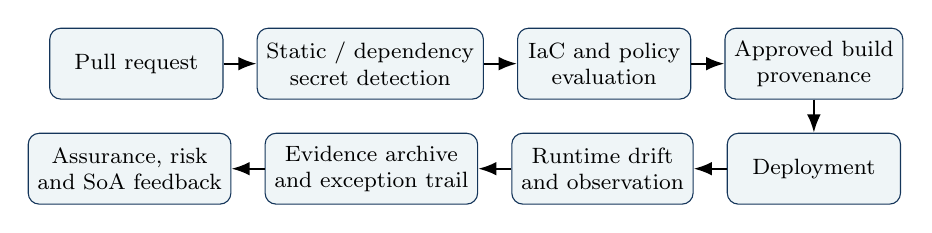
\begin{tikzpicture}[>=Latex,node distance=.42cm, every node/.style={font=\footnotesize}, b/.style={draw=navy,fill=pale,rounded corners,minimum height=.9cm,align=center,minimum width=2.2cm}]
\node[b](a){Pull request};\node[b,right=of a](b){Static / dependency\\secret detection};\node[b,right=of b](c){IaC and policy\\evaluation};\node[b,right=of c](d){Approved build\\provenance};\node[b,below=of d](e){Deployment};\node[b,left=of e](f){Runtime drift\\and observation};\node[b,left=of f](g){Evidence archive\\and exception trail};\node[b,left=of g](h){Assurance, risk\\and SoA feedback};
\foreach \x/\y in {a/b,b/c,c/d,d/e,e/f,f/g,g/h}{\draw[->,thick](\x)--(\y);}
\end{tikzpicture}}\end{center}
\section{Pipeline control gates (example)}
\small\rowcolors{2}{pale}{white}\begin{longtable}{p{.16\linewidth}p{.50\linewidth}p{.28\linewidth}}
\rowcolor{navy} \textcolor{white}{\textbf{Gate}} & \textcolor{white}{\textbf{Sample policy decision}} & \textcolor{white}{\textbf{Risk and evidence}}\\
\endfirsthead
\rowcolor{navy} \textcolor{white}{\textbf{Gate}} & \textcolor{white}{\textbf{Sample policy decision}} & \textcolor{white}{\textbf{Risk and evidence}}\\
\endhead
Code & Required code review and security scan completed for relevant components & 8.4, 8.25, 8.28, 8.29; PR evidence\\
Dependencies & Known severe exposures have assessed exploitability and a risk-based decision & 5.21, 8.8; SBOM, advisory, approval\\
Infrastructure & No prohibited public data store or insecure cryptographic configuration & 8.9, 8.24; IaC diff and policy result\\
Build & Artifact identity and provenance persist into deployment & 8.19, 8.32; attestation and logs\\
Release & Approved branch, authorized actor and environment binding & 8.2, 8.31, 8.32; deployment trace\\
Operations & Sufficient telemetry and recovery evidence for accepted risk & 8.13--8.16; monitors and restore test\\
\end{longtable}\normalsize

\section{Cloud discovery and risk-to-asset joins}
Suggested join graph: \texttt{cloud account} $\rightarrow$ \texttt{resource} $\rightarrow$ \texttt{owner} $\rightarrow$ \texttt{business service} $\rightarrow$ \texttt{classification} $\rightarrow$ \texttt{exposure} $\rightarrow$ \texttt{control finding} $\rightarrow$ \texttt{action} $\rightarrow$ \texttt{evidence}. Normalize ephemeral resource IDs and reconcile deleted assets to prevent reporting false closure. Keep scope changes, scan gaps, exceptions and data source age.
\section{Metrics with denominator discipline}
\begin{itemize}
\item Policy compliance: assessed in-scope cloud resources passing applicable tests / all assessed in-scope resources (report unassessed separately).
\item Remediation timeliness: overdue remediations / all due findings with accepted priorities (do not mix dates across owners).
\item Secrets response time: detection to revocation for verified active credentials, excluding verified benign literals.
\item Evidence integrity: collected artifacts with validated origin and retention / requested in-scope artifacts.
\item Recovery confidence: critical services with successful representative recovery / all critical services requiring test.
\end{itemize}

\section{Operational acceptance examples}
\begin{itemize}
\item A developer cannot use a staging service principal to update production configuration.
\item Terraform changes to public ingress fail a deterministic review rule without exception.
\item Production audit events are delivered to an isolated, access-controlled log service; loss of delivery alerts.
\item A test credential leak cannot be silently committed when prevention is intended and supported.
\item A restore exercise proves recovery of application and authorization configuration, not only data blocks.
\end{itemize}

\clearpage\section*{Source and interpretation policy}
\addcontentsline{toc}{section}{Source and interpretation policy}
\textbf{Source editions:} ISO/IEC 27000:2018 (overview and vocabulary); ISO/IEC 27001:2022 (requirements and normative Annex A); ISO/IEC 27002:2022 corrected 2022-03 (control guidance). Specific clause identifiers are references to the supplied editions, not reproduced control text.\par
\textbf{Interpretation:} ``Source-grounded paraphrase'' describes a concept in the cited source. ``Engineering recommendation'' is a practical model, technology choice, owner, evidence example, frequency, template or scoring convention authored for this suite; it is not a claim that ISO prescribes that exact approach.\par
\textbf{Conformity:} Clauses 4--10 of ISO/IEC 27001 govern ISMS conformity. Applicability of controls is determined through risk treatment, with Annex A used as a completeness cross-check and exclusions justified in the Statement of Applicability (SoA). Source documents alone neither certify an ISMS nor prove control operating effectiveness.\par
\textbf{Source licensing:} Do not distribute or embed the licensed standard PDFs in repositories or distribute copied normative text. Review the editions, amendments, and certification scheme applicable to each assessment before relying on this work.\par
\end{document}
